\mbox{}\\
\vspace{8cm}

This chapter is a reproduction of the following submitted manuscript for publication in GigaScience:

C. I. Mendes, P. Vila-Cerqueira, Y. Motro, J. Moran-Gilad, J. A. Carriço, M. Ramirez. LMAS: Last Metagenomic Assembler Standing

The supplementary information referred throughout the text can be consulted in this chapter before the section of references.

Short-read \ac{SMg} can offer comprehensive microbial detection and characterisation of complex clinical samples. The \textit{de novo} assembly of raw sequence data is key in metagenomic analysis, yielding longer sequences that offer contextual information and afford a more complete picture of the microbial community. The assembly process is the bedrock and may constitute a major bottleneck in obtaining trustworthy, reproducible results.

In this chapter, we present LMAS, an automated workflow developed as a flexible platform to allow users to evaluate traditional and metagenomic dedicated prokaryotic de novo assembly software performance given known standard communities. Its implementation in Nextflow ensures the transparency and reproducibility of the results obtained and the use of Docker containers provides further flexibility. The results are presented in an interactive HTML report where global and reference specific performance metrics can be explored. Currently, 12 assemblers still being maintained are implemented in LMAS, with the possibility of expansion as novel algorithms are developed.

To showcase LMAS we used a test dataset of eight bacterial genomes and four plasmids of the ZymoBIOMICS Microbial Community Standards with linear and logarithmic distribution,  and found that k-mer De Bruijn graph assemblers outperformed the alternative approaches but came with a greater computational cost. Furthermore, assemblers branded as metagenomic specific did not consistently outperform other genomic assemblers in metagenomic samples. Some assemblers still in use, such as ABySS, BCALM2, MetaHipmer2, minia and VelvetOptimiser,  showed significant performance problems and their usability may be limited, particularly when assembling complex samples. 

The performance of each assembler varied depending on the species of interest and its abundance in the sample, with less abundant species presenting a significant challenge for all assemblers. No assembler stood out as an undisputed all-purpose choice for short-read metagenomic prokaryote genome assembly, highlighting that efforts are still needed to further improve metagenomic assembly performance. Our results also suggest that sample complexity and a particular interest in some sample components may affect assembler choice. Using LMAS could help users in their choice of assembler for their specific purpose.  As such, we believe that this manuscript is appropriate for publication in Microbiome as a Software article. 

My contribution to this publication included the design, implementation and optimisation of the LMAS the workflow, including the creation of the Docker containers for all dependencies. I performed the data analysis and comparison of assemblers included in LMAS with ZymoBIOMICS Microbial Community Standards, both evenly and logarithmically distributed samples. Additionally, I've also wrote the manuscript.

\cleardoublepage 

\begin{center}
\large
\textbf{LMAS: Last Metagenomic Assembler Standing}
\end{center}

Catarina I Mendes$^1,*$, 
P Vila-Cerqueira$^1*$,
Y Motro$^2$,
J. Moran-Gilad$^2$,
João A Carriço$^1$
Mário Ramirez$^1$, 


$^1$Instituto de Microbiologia, Instituto de Medicina Molecular, Faculdade de Medicina, Universidade de Lisboa, Lisboa, Portugal 

$^2$Faculty of Health Sciences, Ben-Gurion University of the Negev, Beer-Sheva, Israel

\section{Abstract}

\textbf{Background }The de novo assembly of raw sequence data is key in metagenomic analysis. It allows recovering draft genomes from a pool of mixed raw reads, yielding longer sequences that offer contextual information and provide a more complete picture of the microbial community.
\textbf{Results} To better compare de novo assemblers for metagenomic analysis, LMAS was developed as a flexible platform allowing users to evaluate assembler performance given known standard communities. Overall, in our test datasets, k-mer De Bruijn graph assemblers outperformed the alternative approaches but came with a greater computational cost. Furthermore, assemblers branded as metagenomic specific did not consistently outperform other genomic assemblers in metagenomic samples. Some assemblers still in use, such as ABySS, BCALM2, MetaHipmer2, minia and VelvetOptimiser, perform relatively poorly and should be used with caution when assembling complex samples. 
\textbf{Conclusions} The choice of a de novo assembler depends on the computational resources available, the replicon of interest, and the major goals of the analysis. No single assembler appeared an ideal choice for short-read metagenomic prokaryote replicon assembly, each showing specific strengths. The choice of metagenomic assembler should be guided by user requirements and characteristics of the sample of interest, and LMAS provides an interactive evaluation platform for this purpose. 

\subsubsection{Keywords}

Shotgun Metagenomics, de novo assembly, benchmark, draft genome quality, simulation

\section{Background}

Short-read shotgun metagenomics has the potential to offer comprehensive microbial detection and characterisation of complex clinical or environmental samples.  Despite becoming an increasingly used approach, it comes at the cost of producing massive amounts of data that require expert handling and processing, as well as adequate computational resources. The de novo assembly process is key when analysing metagenomic data since it allows recovering contigs representing the replicons present in the sample, be it genomes, plasmids or bacteriophages, from a pool of mixed raw reads. These contigs are longer sequences that offer better contextual information than reads alone and provide a more complete picture of the microbial community than the species composition. Despite efforts for the development, standardisation and assessment of software for metagenomic analysis, both commercial and open-source \cite{angers-loustau_challenges_2018,gruening_recommendations_2019, sczyrba_critical_2017, couto_critical_2018, meyer_critical_2021}, the de novo assembly process still represents a critical point in these analyses.

The assembly of draft genomes has become a central step when analysing pure bacterial cultures, for instance allowing genomic comparisons through single nucleotide \ac{SNP}s or gene-by-gene methods, such as \ac{cgMLST}. The first assemblers implemented \ac{OLC} approaches, comparing all reads in a sample, computing overlaps and generating consensus sequences by picking the most likely nucleotide for each position in the contigs. As the throughput of sequencing methods increased exponentially, so did the number of pairwise comparisons, limiting the efficiency of these algorithms and making them computationally too expensive. To circumvent this, \ac{dBg} algorithms were increasingly adopted and are currently the most widely used approaches in modern assembly software. Both \ac{OLC} and \ac{dBg} handle unresolvable repeats by essentially fragmenting the sequence, that is, forming multiple contigs for each of the possibly contiguous sequences present in the sample. Additionally, the inherent heterogeneity of complex samples, potentially containing a multitude of replicons, could make traditional genome assemblers, implementing optimisations based on the assumption of having a single genome in the sample, not suitable for metagenomics \cite{ayling_new_2020}.

Several dedicated metagenomic assembly tools for short-read data are available \cite{ayling_new_2020}. These tools are generally assumed to perform better when dealing with complex samples having a combination of intragenomic and intergenomic repeats and uneven and low coverage sequencing depths of some of the replicons \cite{olson_metagenomic_2019}. Not using dedicated metagenomic assemblers was suggested to come with the cost of generating artificial variation and chimeric contigs, especially in samples that contain closely related species \cite{teeling_current_2012}. However, to our knowledge, no formal comparison has been done looking at increased accuracy or gains in contiguity of assemblies obtained with metagenomic assemblers versus traditional assemblers.

With an ever-increasing range of both traditional and metagenomic assemblers becoming available, choosing the best performing tool can be an arduous and time-consuming task since the choice may vary depending on the purpose of the analysis, organism of interest, complexity of the sample and computational infrastructure available. Additionally, the evaluation of the resulting contigs is not straightforward since one metric is not sufficient to classify an assembly, particularly with complex samples \cite{olson_metagenomic_2019,bradnam_assemblathon_2013}. Despite several de novo assembly validation methods relying on features of the created contigs themselves, such as QUAST \cite{gurevich_quast_2013}, being useful in identifying inconsistencies indicative of potential assembly errors, the use of reference-based validation methods offer the possibility of a more complete evaluation of accuracy and are particularly important to benchmark attempts to reconstruct communities. MetaQUAST \cite{bradnam_assemblathon_2013}, a modification of QUAST, extends the original software by performing assembly evaluation based on aligning contigs to a reference, which can be provided or inferred by the software, and reports, in addition to the standard metrics for single genomes reported by QUAST, the number of interspecies translocations and the number of possibly misassembled contigs.

The use of mock communities, with known composition, abundance and genomic information, provides a ground truth against which the success of the assembly of a complex sample can be evaluated. Such mock communities facilitate the identification of misassemblies, such as chimeric sequences generated from the improper combination of two distinct replicons, indels or single nucleotide variants improperly created by the assembler. On the other hand, the comparison of the performance of two assemblers is only possible if the input data is the same and if the same evaluation metrics are applied \cite{sczyrba_critical_2017}. 

To tackle these challenges, we developed LMAS (Last Metagenomic Assembler Standing), an automated workflow to enable the benchmarking of traditional and metagenomic prokaryotic de novo assembly software using defined mock communities. The results of LMAS are presented in an interactive HTML report where selected global and reference replicon specific performance metrics can be explored. The mock communities can be provided by the user to better reflect the samples of interest. New assemblers can be added with minimal changes to the pipeline so that LMAS can be expanded to include novel algorithms as they are developed. The portability and ease of use of LMAS is intended to allow users to evaluate the performance of assemblers in mock communities, mimicking as closely as possible their samples of interest. LMAS is open source and the workflow and its documentation are available at \url{https://github.com/B-UMMI/LMAS} and \url{https://lmas.readthedocs.io/} respectively. 

\section{Implementation}

\subsection{Workflow overview}

LMAS is a user-friendly automated workflow enabling the benchmarking of traditional and metagenomic prokaryotic de novo assembly software using defined mock communities. LMAS was implemented in Nextflow [12]\cite{di_tommaso_nextflow_2017} to provide flexibility and ensure the transparency and reproducibility of the results. LMAS relies on the use of Docker \cite{merkel_docker_2014} containers for each assembler, allowing versions to be tracked and changed easily.

\newpage

\begin{figure*}[h!]
\centering
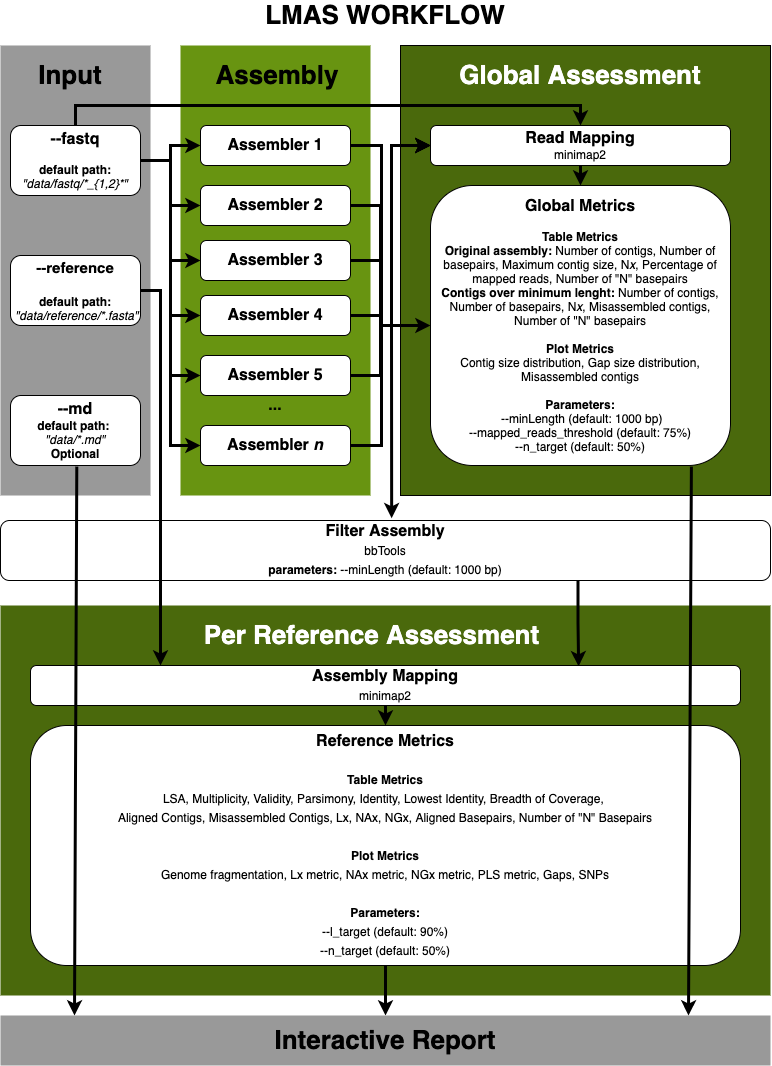
\includegraphics[width=\textwidth]{figures/chapter 5/Figure 1.png}
\caption{The LMAS workflow. The input sequencing data is assembled in parallel, resources permitting, by the set of assemblers included in LMAS. The resulting contigs are processed and the global quality assessment is performed. After filtering for the user-defined minimum contig size, the remaining sequences are mapped against the provided reference and the resulting information is processed to evaluate assembly quality by replicon in the reference file. All results, and optional text information describing the samples, are grouped in the LMAS report.}
\label{fig:chap5_figure1}
\end{figure*}

\newpage

\subsection{Installation and Usage}

LMAS can be installed through Bioconda \cite{noauthor_lmas_nodate} or Github \cite{mendes_lmas_2021}, with detailed instructions available in the documentation \cite{noauthor_installation_nodate}. LMAS requires as inputs the complete reference replicons (genomes, plasmids or any other replicons present) and short-read paired-end raw data. All complete references (linear replicons) should be provided in a single file. This raw data can be either obtained in silico by creating simulated reads from the reference replicons or sequencing mock communities of known composition. Optionally, information on the input samples in a markdown file can be provided to be presented in the report.

A step-by-step execution tutorial is available at \cite{noauthor_basic_nodate}. Users can customise the workflow execution either by using command-line options or by modifying the simple plain-text configuration files. To make the execution of the workflow as simple as possible, a set of default parameters and directives is provided. A complete description of each parameter is available in Supplemental Material (see Supplemental Material, Workflow parameters), as well as in the documentation \cite{noauthor_parameters_nodate}.  The results are presented in an interactive HTML report, stored in the “report” folder in the directory of LMAS’ execution. The output files of all assemblers and quality assessment processing scripts in the workflow are stored in the “results” folder, in the same location. 

\subsection{Supported Assemblers and selection criteria}

A collection of de novo assembly tools was compiled, including OLC and dBg assembly algorithms, the latter including both single k-mer and multiple k-mer value approaches, and hybrid assemblers implementing both algorithms, including both genomic and metagenomic assemblers (Supplemental Table S1). Of these, 12 assemblers were selected based on the date of last update and are implemented in LMAS: ABySS \cite{jackman_abyss_2017} (version 2.3.1), BCALM2 \cite{chikhi_compacting_2016} (version 2.2.3), GATB Minia Pipeline \cite{noauthor_gatbgatb-minia-pipeline_2022} (commit hash 9d56f42) , IDBA-UD \cite{peng_idba-ud_2012} (version 1.1.3), MEGAHIT \cite{li_megahit_2015} (version 1.2.9), MetaHipMer2 \cite{georganas_extreme_2018} (version 2.0.0.65-gaad446d-dirty-AddGtest), metaSPAdes \cite{nurk_metaspades_2017} (version 3.15.3), minia \cite{chikhi_space-efficient_2013} (version 3.2.6), SKESA \cite{souvorov_skesa_2018} (version 2.5.0), SPAdes \cite{bankevich_spades_2012} (version 3.15.3), Unicycler \cite{wick_unicycler_2017} (version 0.4.9) and VelvetOptimiser \cite{seemann_velvetoptimiser_2021} (commit hash 092bdee) (Table \ref{tab:ch5_table1}). The execution commands for each assembler are available as Supplemental Material (see Supplemental Material, Short-read de novo assemblers) and in the documentation \cite{noauthor_short-read_nodate}. 
New assemblers can be added with minimal changes to the pipeline so that LMAS can be expanded as novel algorithms are developed. A template is available to facilitate their integration and a step-by-step guide is included in the documentation \cite{noauthor_add_nodate}. The only two requirements for the addition of a new assembler are the execution command for the assembler for paired-end short-read data and a Nextflow-compatible container with the assembler and any dependencies.

\begin{scriptsize}
\begin{center}

\begin{table}[]
\centering
\caption{Prokaryotic de novo assemblers integrated into LMAS.}
\label{tab:ch5_table1}
\begin{tabular}{@{}lll@{}}
\toprule
Assembler         & Type        & Algorithm                        \\ \midrule
GATBMiniaPipeline & Metagenomic & Multiple   k-mer De Bruijn graph \\
IDBA-UD           & Metagenomic & Multiple   k-mer De Bruijn graph \\
MEGAHIT           & Metagenomic & Multiple   k-mer De Bruijn graph \\
MetaHipMer2       & Metagenomic & Multiple   k-mer De Bruijn graph \\
metaSPAdes        & Metagenomic & Multiple   k-mer De Bruijn graph \\
ABySS             & Genomic     & Single   k-mer De Bruijn graph   \\
BCALM2            & Genomic     & Single   k-mer De Bruijn graph   \\
MINIA             & Genomic     & Single   k-mer De Bruijn graph   \\
SKESA             & Genomic     & Multiple   k-mer De Bruijn graph \\
SPAdes            & Genomic     & Multiple   k-mer De Bruijn graph \\
Unicycler         & Genomic     & Multiple   k-mer De Bruijn graph \\
VelvetOptimizer   & Genomic     & Multiple   k-mer De Bruijn graph \\ \bottomrule
\end{tabular}
\end{table}

\end{center}
\end{scriptsize}


\subsection{Assembly Quality Metrics}

The success of an assembly is evaluated in two steps: globally (see \ref{sssec:_chap5_global_metrics}) and relative to each of the replicons present in the sample (see \ref{sssec:_chap5_reference_metrics}). In both, the tabular presentation in the reports allows the comparison of exact values between assemblers, and the interactive plots allow a more intuitive overview and easy exploration of results. In addition to the assembly success metrics, computational resource statistics are registered for each assembler (see Supplemental Material, LMAS Metrics, Computational Performance Metrics).

\subsubsection{Global Metrics} \label{sssec:_chap5_global_metrics} 

The computation of the global metrics is performed through statistics inherent to the complete set of contigs assembled per sample, independent of the species/sample of origin. The metrics are presented, in tabular form, for the complete set of contigs and those filtered for a minimum length, and also graphically for the contigs filtered for a minimum length. The statistics include information on contig number, size and ambiguous bases; and the proportion of reads mapping to the created contigs. Two statistics are a consolidation of per reference metrics: misassemblies (i.e. contigs that do not reflect the structural organisation in the reference replicons); and the overall size of gaps in all reference replicons not covered by any contig. A more detailed description of all global metrics is available in Supplemental Material (see Supplemental Material, LMAS Metrics, Global Metrics). 

\subsubsection{Per Reference Metrics} \label{sssec:_chap5_reference_metrics} 

For the computation of the reference-based metrics, only the filtered set (FS) contigs are considered, for each reference replicon in the sample. These contigs are the ones exceeding the user-defined minimum sequence length, filtered using BBTools (version 38.44). After this initial step, the contigs are mapped to the reference replicons with minimap2 \cite{li_minimap2_2018} (version 2.22). The metrics are computed through custom python code (see Supplemental Material, Assembly filtering and mapping) for each replicon in the file provided as input. A detailed description of all reference-based metrics is available in Supplemental Material (see Supplemental Material, LMAS Metrics, Per Reference Metrics). 

In addition to the statistics shared with the global metrics, LMAS also calculates the number of mismatches relative to each reference, the COMPASS \cite{earl_assemblathon_2011} metrics and two new metrics we propose: LSA and Pls.

LSA represents the fraction of the longest single alignment between a contig and the reference, relative to the reference length. The Pls, or Phred-like score, is a scoring function based on the identity of each aligned contig to the reference replicon. Similarly to the Phred quality score \cite{ewing_base-calling_1998}, a measure of the quality of the identification of the bases by sequencing, the Pls measures the quality of the assembly of a contig. The formula of Pls is similar to the Phred score formula but uses as the error function the identity of the base in the contig to that of the reference replicon. The formula to obtain the Pls metric per contig is Equation \ref{ch5_eq1}. 

\begin{equation} \label{ch5_eq1}
    Phred(E) = \left\{\begin{matrix}
-log(E)\times 10 & \textup{if }E < 60\\ 
 60 & \textup{if }E = 60
\end{matrix}\right. \\
\textup{ where }E = 1-\textup{Identity}
\end{equation}

\subsection{The LMAS Report}

The LMAS results are presented in an interactive HTML. The LMAS report is composed of two main panels: a top summary panel with information on input samples (provided by the user) and the resources used during LMAS’ execution, and a bottom panel where selected global and reference specific assembly metrics can be explored for each sample. LMAS constructs the HTML file after workflow completion, storing it in the “reports” folder. The report data can be easily shared between users and requires only a browser for visualisation.

\begin{figure*}[h!]
\centering
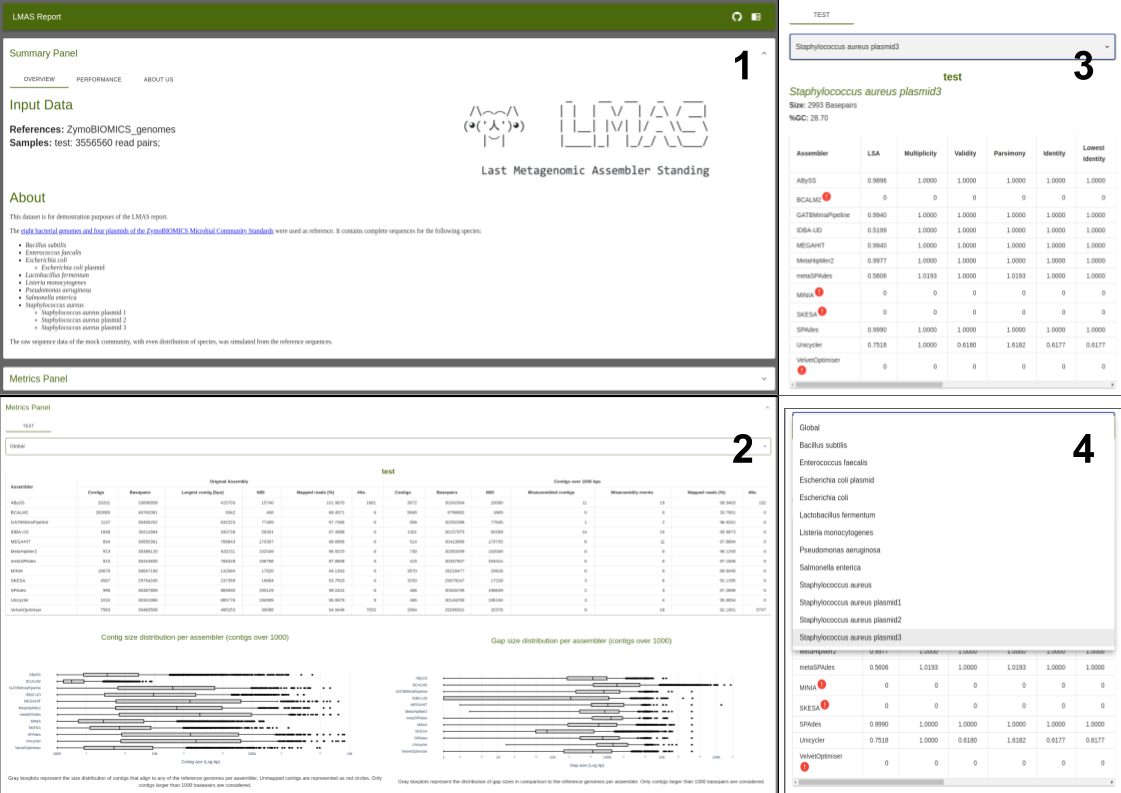
\includegraphics[width=\textwidth]{figures/chapter 5/Figure 2.png}
\caption{The LMAS report.  All results, and optional text information describing the samples, are grouped in the LMAS report, an interactive and responsive HTML file,  for exploration in any browser. Links for LMAS source code and documentation are available in the top right corner of the report. 1) The summary panel of the LMAS report contains information on the input reference sequences and raw sequencing data samples (provided by the user), and the overall computational performance of the assemblers in LMAS. 2) The LMAS metric panel contains the explorable global and reference specific performance metrics per input raw sequencing data sample.  The tabular presentation allows direct comparison of exact values between assemblies, and the interactive plots allow for an intuitive overview and easy exploration of results. 3) If an assembler fails to produce an assembly, or fails to assemble sequences that map to the reference replicon, it is marked in the table with a red warning sign. 4) The global or reference replicon specific metrics can be accessed for each sample in the dropdown menu.}
\label{fig:chap5_figure2}
\end{figure*}

\subsubsection{Summary Panel} \label{sssec:_chap5_summary_panel}

The top panel of the report contains information on the input samples and overall performance of the assemblers in LMAS, divided into three tabs:  Overview, Performance and About us. On the top right corner of the report, direct links to LMAS’ source repository and documentation are provided.

\begin{itemize}
    \item \textit{Overview}: This tab contains information on the input data, including the name and number of reads of the raw sequencing data, and the name of the reference file. Additional information provided by the user about the community used as input is also presented here. 
    \item \textit{Performance}: This tab contains a table with information on the version, the containers used and computational performance metrics for each assembler in LMAS.
    \item\textit{ About us}: This tab contains information on the LMAS GitHub repositories and the LMAS development team. 
\end{itemize}

\subsubsection{}{Metrics Panel} \label{sssec:_chap5_summary_panel} 

The bottom portion of the report contains the explorable global and reference specific performance metrics per input raw sequencing data sample. Each sample has its own tab and the global or reference replicon specific metrics can be accessed in the dropdown menu. 


\paragraph{Global Metrics} \label{sssec:_chap5_summary_panel_global} \mbox{}\\

A table displays the global assembly metrics computed for the complete and FS contigs. If an assembler fails to produce an assembly, it is marked on the table with a red warning sign. The global metric plots are interactive, allow zooming in on particular areas and provide extra information as hover text boxes. The plots can be saved as PNG in whatever view the user selects. 

\paragraph{Per Reference Metrics} \label{sssec:_chap5_summary_panel_reference} \mbox{}\\

Similarly to the global assembly metrics, a table displays the computed set of reference restricted metrics for the FS contigs. If an assembler fails to produce sequences that align to the reference, these are marked in the table with a red warning sign. Information on the expected reference replicon length and the GC content is calculated from the input files and reported above the table. The per-reference metric plots are also interactive, allowing the same type of operations as the global metric plots. 

\subsection{Comparison with other assembly evaluation software programs}

The assessment and evaluation of genome assemblies has been a relevant field ever since the emergence of the assembly process itself, and therefore many solutions have been proposed \cite{sczyrba_critical_2017, olson_metagenomic_2019, bradnam_assemblathon_2013, gurevich_quast_2013, mikheenko_metaquast_2016, manchanda_genomeqc_2020, meader_genome_2010, challis_blobtoolkit_2020}. The Critical Assessment of Metagenome Interpretation (CAMI) proposed a set of recommendations and best practices for benchmarking in microbiome research \cite{meyer_tutorial_2021}. These recommendations include the reporting of computational performance, which may condition the choice of software by the users, such as runtime, disk space and memory consumption, also reported by  LMAS (see Supplementary Material, LMAS Metrics). As also suggested by CAMI, LMAS tracks the exact program version and command-line calls through its implementation in Nextflow. Moreover,  using containerised assemblers and being easily installable through Bioconda, LMAS facilitates deployment in diverse user machines. Unlike the CAMI tutorial, in which users are asked to download and install the necessary tools, in LMAS everything is provided in a one-stop reproducible workflow that effortlessly handles all pre-processing, assembly, post-processing, traceability and report production steps, freeing users to focus on providing relevant samples for analysis and interpreting the results in view of the intended applications.

Concerning software for assembly quality assessment currently available, the most widely adopted is QUAST \cite{gurevich_quast_2013}, or when dealing with metagenomic data, its extension metaQUAST \cite{mikheenko_metaquast_2016}, which was also adopted by the CAMI challenges [3,5] \cite{sczyrba_critical_2017, meyer_critical_2021} and suggested in the CAMI Tutorial \cite{meyer_tutorial_2021}. Although several features of these tools overlap with LMAS’ quality assessment components, these differ from LMAS in the sense that they are not a single step workflow allowing a traceable and reproducible assembly of mock communities. Unlike QUAST and metaQUAST, whose purpose is to evaluate assemblies, the purpose of LMAS is to allow users to evaluate assembler performance for a given sample of interest. Supplementary Table S2 shows the comparison of the output and computed assembly quality metrics generated by LMAS, QUAST and metaQUAST. 

\section{Results and Discussion}

To illustrate the use of LMAS and evaluate the performance of the chosen assemblers we used the eight bacterial genomes and four plasmids of the ZymoBIOMICS Microbial Community Standards as reference. As input we used the raw sequence reads of mock communities with an even and logarithmic distribution of species, from real sequencing runs \cite{nicholls_ultra-deep_2019} and simulated read datasets, with and without error, matching the distribution of species in each sample \cite{gourle_simulating_2019}. Our dataset is composed of samples ENN (in silico generated evenly distributed without error), EMS (in silico generated evenly distributed with Illumina MiSeq error model), ERR2984773 (evenly distributed real Illumina MiSeq sample), LNN (in silico generated logarithmically distributed without error), LHS (in silico generated logarithmically distributed with Illumina HiSeq error model) and ERR2935805 (logarithmically distributed real Illumina HiSeq sample) (see Supplemental Table S3). Detailed information about the generation of the input samples is available as Supplemental Material (see Supplemental Materials, ZymoBIOMICS microbial community standards, Supplemental Table S4). To evaluate the reproducibility of an assembler performance, the LMAS workflow was run three times for all samples using default parameters, and the resulting data was processed for each sample (see Supplemental Materials, Assessment of Assembly Success) Supplementary Table S5 to Table S10 present an overview of the average global performance per assembler for each sample in LMAS. 

\subsection{Some assemblers perform poorly}

Of the 12 de novo prokaryotic assemblers included in LMAS, five stand out as having an overall poor performance: ABySS, BCALM2, MetaHipmer2, minia and VelvetOptimiser. Both ABySS and MetaHipmer2 performed inconsistently with differing resource requirements for the same sample in different runs, namely run time and memory allocation (see Supplemental Materials, Resource Requirements Differ Greatly, Supplemental Figure S2).  Moreover, ABySS failed to produce an assembly for sample ERR2984773 for 1 of the runs (see Supplementary Table S7) and for sample LHS in any of the 3 runs in the time limit of 3 days (see Supplementary Table S9), and MetaHipmer2 failed to produce an assembly for samples LNN and LHS in all 3 runs (see Supplementary Tables S8-S9). VelvetOptimiser generated the highest number of inconsistent contigs across the 3 LMAS runs (Figure \ref{fig:chap5_figure3}, Supplementary Table S11), with 1.69\% of the total contigs created present in only 1 or 2 runs. Although not as extreme as VelvetOptimiser, ABySS (0.52\%), minia (0.14\%), GATBMiniaPipeline (0.32\%), MetaHipMer2 (0.11\%) and IDBA-UD (0.08\%) also showed inconsistencies in contig size.

\begin{figure*}[h!]
\centering
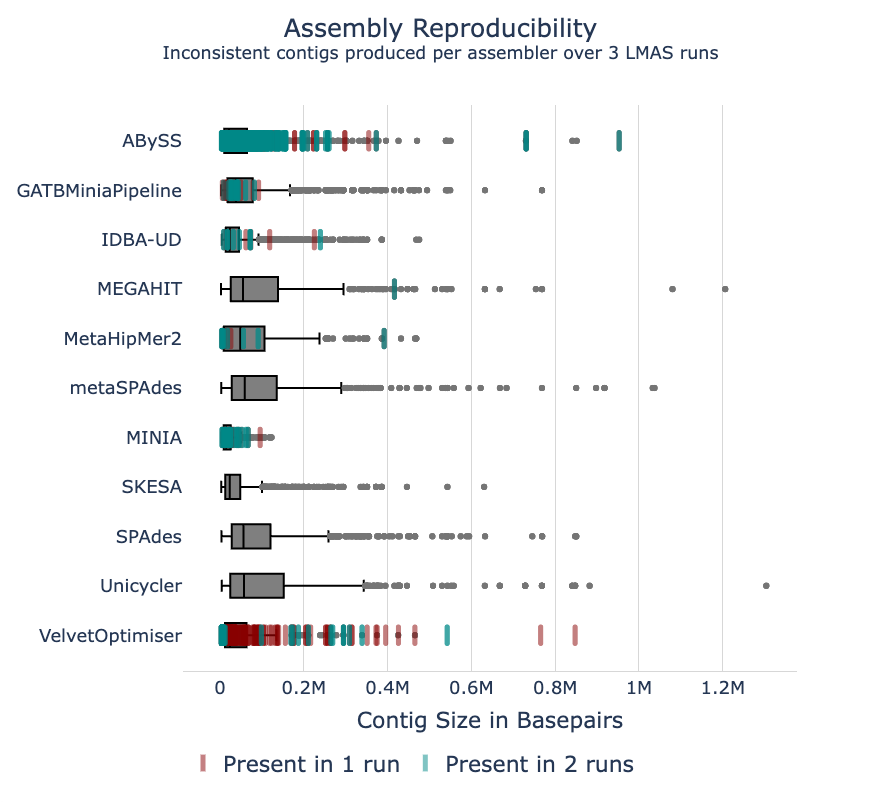
\includegraphics[width=\textwidth]{figures/chapter 5/Figure 3.png}
\caption{Assembly robustness. Inconsistent contigs produced per assembler over 3 LMAS runs. The distribution of contig sizes, in basepairs, consistently present in all three LMAS runs are indicated in the grey boxplots for each assembler. If an assembler produced a contig only present in two of the runs (as determined by its size), its size is indicated in teal. If a contig is present in a single run, it is represented in red.}
\label{fig:chap5_figure3}
\end{figure*}

Regarding the quality assessment of the assemblies produced (Figure \ref{fig:chap5_figure4}, Supplementary Table S12), ABySS, BCALM2 and minia are the only single k-mer dBg assemblers in the collection and were found to mostly underperform relative to their multiple k-mer dBg counterparts, generally resulting in more fragmented assemblies, although there were significant differences in performance across samples. Among multiple k-mer assemblers, VelvetOptimiser frequently produced a very high number of contigs of very small size (over 99\% of the contigs not surpassing the minimum length of 1,000 bp) and therefore a low N50 (an average of 29,768 bp versus a global average of 84,114 bp) (Supplementary tables S5-S10). Additionally, ABySS and VelvetOptimizer produced contigs with a very large number of Ns, with an average of 1,019 and 3,035 uncalled bases per assembly, respectively. MetaHipMer2, although having overall average metrics in the two evenly distributed mock samples (ENN and EMS, Supplementary Tables S5-S6) where it was able to run successfully, it severely underperformed in the real samples (ERR2984773 and ERR2935805, Supplementary Tables S7 and S10). Generally, the performance scores of the assemblers decreased considerably for the real samples in comparison with the simulated ones, either with or without error. High utilisation of the reads in the dataset is observed for most assemblers, with on average at least 90\% of the reads mapping back to the assembly, except for ABySS, BCALM2, MetaHipMer2 and VelvetOptimiser whose values are in the range of 46-79\%. Despite an overall good performance, SPAdes produced the highest number of misassembled contigs, with an average of 98 and a maximum of 572 (sample ERR2935805, Supplementary Table S10), in comparison to the global average of 11 misassembled contigs for all assemblers across all samples.

Due to their poor performance discussed above, the following assemblers have not been included in subsequent analyses: ABySS, BCALM2, MetaHipmer2, minia and VelvetOptimiser. 

\begin{figure*}[h!]
\centering
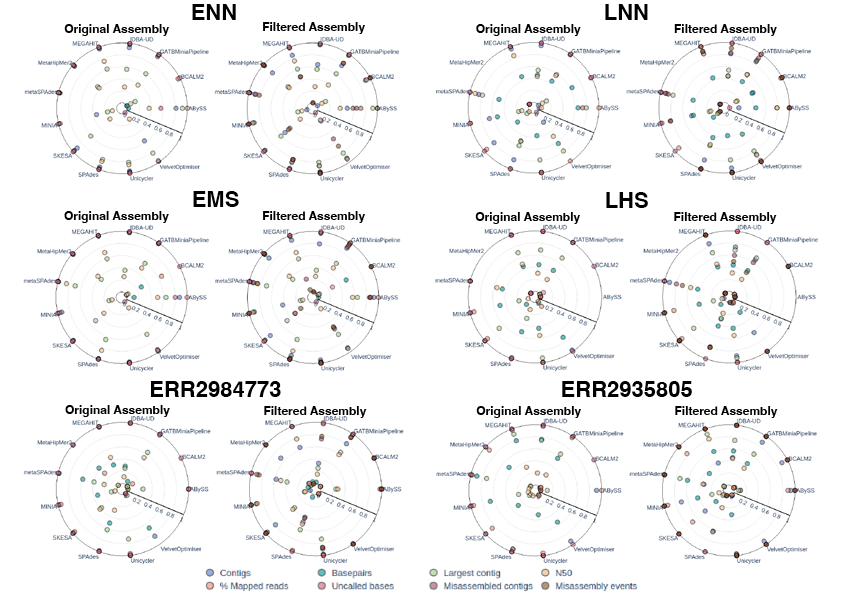
\includegraphics[width=\textwidth]{figures/chapter 5/Figure 4.png}
\caption{Assembler performance for the ZymoBIOMICS Microbial Community Standards dataset. For each sample in the dataset, the best score of each assembler in the 3 LMAS runs was selected. The results for each global assembly metric was normalised, with 1 representing the best result, and 0 the worst. For the original assembly, the following metrics are presented: number of contigs produced (in blue), number of basepairs produced (in teal), the size of the largest contig assembled (in green), N50 (in yellow), percentage of mapped reads to the assembly (in orange) and uncalled bases (in red).  For the filtered assembly, the additional metrics are presented: number of misassembled contigs (in purple) and number of misassembly events (in brown). }
\label{fig:chap5_figure4}
\end{figure*}

\subsection{Metagenomic dedicated assemblers do not outperform genomic assemblers}

After excluding the poorly performing assemblers, LMAS includes 3 genomic (SKESA, SPAdes and Unicycler) and 4 labelled as metagenomic specific (GATBMiniaPipeline, IDBA-UD, MEGAHIT and metaSPAdes) de novo prokaryotic assemblers, all implementing multiple k-mer dBg algorithms. As observed in Figure \ref{fig:chap5_figure5}, Supplementary Table S13 and Supplemental Figure S3,  there were very significant differences between the best and the worst performing assemblers of each type, with this difference being more pronounced for metagenomic assemblers. The best performing assemblers of each type behaved frequently quite similarly, and the differences between them tended to be attenuated after filtering for contigs <1 kbp. Still, for the linearly distributed samples (ENN, EMS and ERR2984773), the overall worst performers tended to be metagenomic assemblers. In contrast, for the logarithmically distributed samples (LNN, LHS and ERR2935805) the opposite was observed, with genomic assemblers tending to be the worst-performing (Figure \ref{fig:chap5_figure5}). For the logarithmically distributed samples, the number of basepairs recovered is significantly lower than expected from their composition for both genomic and metagenomic assemblers, particularly after filtering (Supplementary Table S13), as contigs representing the less abundant species are not recovered by either type of assemblers (see Assembler performance is influenced by replicon abundance in the sample). For this dataset, the fact that an assembler is branded as genomic or metagenomic does not translate into better or worse performance in dealing with these complex samples, but rather characteristics of the individual assemblers themselves determine their performance.

\begin{figure*}[h!]
\centering
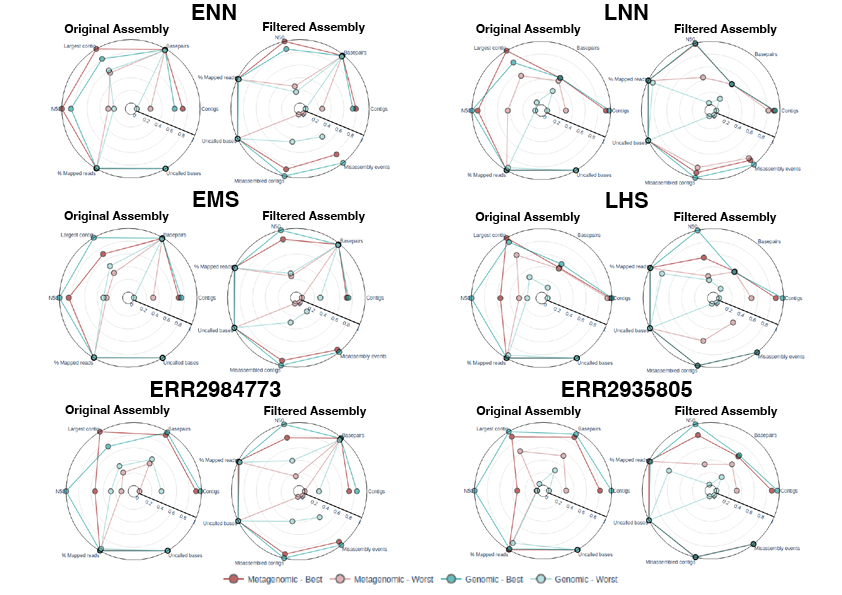
\includegraphics[width=\textwidth]{figures/chapter 5/Figure 5.png}
\caption{Performance of genomic and metagenomic assemblers for the ZymoBIOMICS Microbial Community Standards dataset. For each sample in the dataset and for the 3 runs, the best and worst scores for each assembler category were selected: genomic (in blue) and metagenomic (in red). The results for each global assembly metric were normalised, with 1 representing the best result, and 0 the worst. For the original assembly, the following metrics are presented: number of contigs produced, number of basepairs produced, the size of the largest contig assembled, N50, percentage of mapped reads to the assembly and uncalled bases.  For the filtered assembly, the additional metrics are presented: number of misassembled contigs and number of misassembly events.}
\label{fig:chap5_figure5}
\end{figure*}

\subsection{Success is not straightforward}

Several factors contribute to suboptimal performance of the assembly process, from DNA isolation and library preparation protocol; sequencing technology, depth and read length; to possible contamination and inherent characteristics of the sample composition.

\subsubsection{Assembler performance is influenced by species}